 % Referencia: MDA. Engeenering emergency (dorman's)

% ---------------------------------------------------------------------------- %
\chapter{Conceitos, Técnicas e Ferramentas}
\label{cap:conceitos_tecnicas_e_ferramentas}
% ---------------------------------------------------------------------------- %

Assim como no processo de desenvolver um software, um jogo possui vários conceitos e ferramentas próprias que ajudam na comunicação e organização durante o desenvolvimento.
Para familiarizar o leitor com as técnicas e jargões normalmente utilizados, é descrito nesse capítulo um pouco da linguagem específica no mundo de \textit{game development}, além das técnicas e ferramentas específicas que foram utilizadas na criação de \textit{PsyChO: The Ball}.

% ---------------------------------------------------------------------------- %
\section{Conceitos}
\label{sec:conceitos}
A interatividade de um jogo consiste em quais ações um usuário pode realizar e de que forma isso altera o estado atual do jogo. Essa dinâmica define a jogabilidade de um jogo virtual, também chamada de \textit{gameplay}. Os tipos de interações que o jogador tem acesso são denominadas \textit{mecânicas} do jogo e estas variam dependendo de qual experiência você deseja transmitir para o usuário.

Exemplificando, em jogos de plataforma 2D clássicos como \textit{Super Mario Bros.} para \textit{Nintendo Entertainment System}\cite{mario}, o jogador controla um personagem que precisa pular e atravessar obstáculos até terminar o jogo. Para isso, o usuário pode correr e pular, mecânicas fornecidas para enfrentar os desafios propostos. Esses recursos, juntos ao \textit{feedback} que o próprio jogo retorna, geram uma \textit{experiência} para o jogador, objetivo principal da criação de jogos.

A área de estudo sobre a criação de experiências em jogos se denomina \textit{Game Design}. O \textit{game designer} Jesse Schell a define em seu livro sobre o assunto \cite{jessegamedesign} da seguinte forma:

\begin{displayquote}
  \textit{Game Design é o ato de decidir como um jogo deve ser.}\footnote{Tradução livre feita pelo autor}
\end{displayquote}

É natural esperar que essa área não seja uma ciência exata, de forma que não existe algoritmos ou fórmulas matemáticas que definem exatamente como fazer um jogo "bom". Muito pelo contrário, o estudo na área de Game Design é um conjunto de idéias e linhas de pensamento para auxiliar no desenvolvimento de jogos e mais facilmente transmitir a experiência desejada pelo desenvolvedor. Também no mesmo livro\cite{jessegamedesign}, Schell cria um sistema de "lentes", cada uma representando alguma visão ou crítica para analisar as mecânicas e funcionalidades de um jogo e averiguar a consistência entre experiência desejada e transmitida.

Como temos esse objetivo final de \textit{experiência para o usuário}, é muito comum a utilização de documentos para formalmente especificar e detalhar como será o desenvolvimento do jogo. Um documento famoso desse tipo é o \textit{Game Design Document} ou \textit{GDD}. Seu objetivo é servir como uma "receita de bolo", determinando o gênero do jogo, suas mecânicas, detalhamentos de personagens ou roteiro da história, ou até uma breve descrição do que é seu jogo, de forma que todos que trabalhem no projeto possam facilmente consultar e utilizar como guia durante o desenvolvimento. Em seu livro de Fundamentos em Game Design \cite{ernestgamedesign}, Ernest Adams descreve Game Design Documents da seguinte forma:

\begin{displayquote}
  \textit{Os documentos gravam decisões feitas e concordadas oralmente [entre os integrantes do grupo]; (...) mais importante que isso, eles transformam ideias vagas em planos explícitos.}\footnote{Tradução livre feita pelo autor}
\end{displayquote}

Desta forma, apesar de parecer um gasto adicional de tempo sem grandes benefícios, a manutenção de documentos de design acaba poupando tempo em resolução de conflitos de ideias e deixa o desenvolvimento de um jogo muito mais fluído. Para o jogo \textit{PsyChO: The Ball} foi criado um documento que brevemente descreve sua jogabilidade e gênero.

No caso, \textit{PsyChO: The Ball} é considerado um \textit{Top Down Shooter}, um gênero muito famoso em jogos onde o jogador controla um personagem que precisa se esquivar de inimigos e atirar projéteis para se defender. Além disso, a visão do jogo é de cima pra baixo, observando todos elementos do jogo pelo topo.

Na parte prática de desenvolvimento necessitamos de ferramentas para produzir e gerar o jogo. Estas são chamadas de \textit{Motores de Jogos} ou \textit{Game Engines}. Uma \textit{Game Engine} consiste em várias bibliotecas que auxiliam na produção de um jogo, além de alguma estruturação para gerenciar e manipular elementos lógicos. Elas possuem métodos para desenhar objetos na tela, reproduzir arquivos de sons, lidar com \textit{input} de usuário e, em muitos casos, outras funcionalidades úteis, como métodos para simular interações físicas ou gerenciar janelas. Uma versão mais simples de uma \textit{Game Engine} é uma \textit{Framework} ou \textit{Arcabouço}. Esta também é um conjunto de bibliotecas, mas geralmente mais abertas e sem uma estrutura rígida para desenvolver o jogo.

Mas seja uma Game Engine ou um Arcabouço, todas ferramentas para criação de jogos utilizam um laço lógico chamado de \textit{Game Loop}. Cada ferramenta tem sua própria versão e implementação, mas em geral todas tem 3 pontos chave: processar \textit{inputs}, atualizar objetos no jogo e renderizar elementos gráficos. Podemos visualizar esse laço da seguinte forma, como visto no segundo capítulo do livro de Robert Nystrom, Game Programming Patterns \cite{robertgameloop}:

\begin{lstlisting}
  while (true)
  {
    processInput();
    update();
    render();
  }
\end{lstlisting}

A função \textit{processInput} é responsável por verificar se o usuário pressionou alguma tecla ou de algum modo fez algo no mundo físico que afete o jogo. A função \textit{update} é responsável pela parte lógica do jogo, como atualizar as posições de inimigos, determinar colisões e qualquer outra atualização lógica necessária. É muito comum que essa função receba um argumento especial que diz quanto tempo se passou desde a última chamada dela (muitas vezes denominado de \textit{dt}). Assim é possível fazer cálculos relativos ao tempo de forma mais realista. Por último, a função \textit{render} é responsável por desenhar os objetos na tela, normalmente apagando o que foi desenhado anteriormente.


% ---------------------------------------------------------------------------- %
\section{Técnicas}
\label{sec:tecnicas}

Apesar de grande parte do desenvolvimento de \textit{PsyChO: The Ball} ter sido feita apenas por uma pessoa, foi muito benéfica a utilização de sistemas de versionamento que ajudam tanto na centralização de todo o código do jogo, facilitando na transição entre ambientes de trabalho, quanto na possibilidade de guardar versões antigas e resgatar códigos passados quando necessário. Durante todo o desenvolvimento de \textit{PsyChO: The Ball} foi utilizado um sistema de controle de versão para código e nele se encontra todas as versões de lançamento do jogo.

Uma boa prática na produção de um jogo, seja esse comercial ou um projeto pessoal, é a de \textit{releases constantes}. O propósito disto é ter, periodicamente, lançamento de versões estáveis e jogáveis do jogo, de forma que outras pessoas possam jogar e dar \textit{feedback} frequente, assim ajudando no encaminhamento do projeto. Essa técnica é muito comum em metodologias ágeis de desenvolvimento de software e essa linha de pensamento foi o que guiou todo o desenvolvimento de \textit{PsyChO: The Ball}.

Inicialmente foi utilizado o sistema \textit{Kanban}, uma abordagem moderna de conceitos ágeis muito comum em empresas ou grupos de desenvolvimento de software. Kleber Bernardo, especialista em métodos ágeis, descreve bem o método em um artigo no site Cultura Ágil \cite{kleberkanban}:

\begin{displayquote}
  \textit{O Kanban lhe ajuda a assimilar e controlar o progresso de suas tarefas de forma visual. É, normalmente, utilizado um quadro branco com alguns pequenos papéis (Post-it) colados, esses papéis representam as suas tarefas, ao termino de cada tarefa o papel é puxado para a etapa seguinte até que a mesma seja finalizada. Ao olhar para um quadro Kanban é fácil enxergar como o trabalho seu e de sua equipe fluem, permitindo não só comunicar o status, mas também dar e receber feedbacks.}
\end{displayquote}

\begin{figure}[h!]
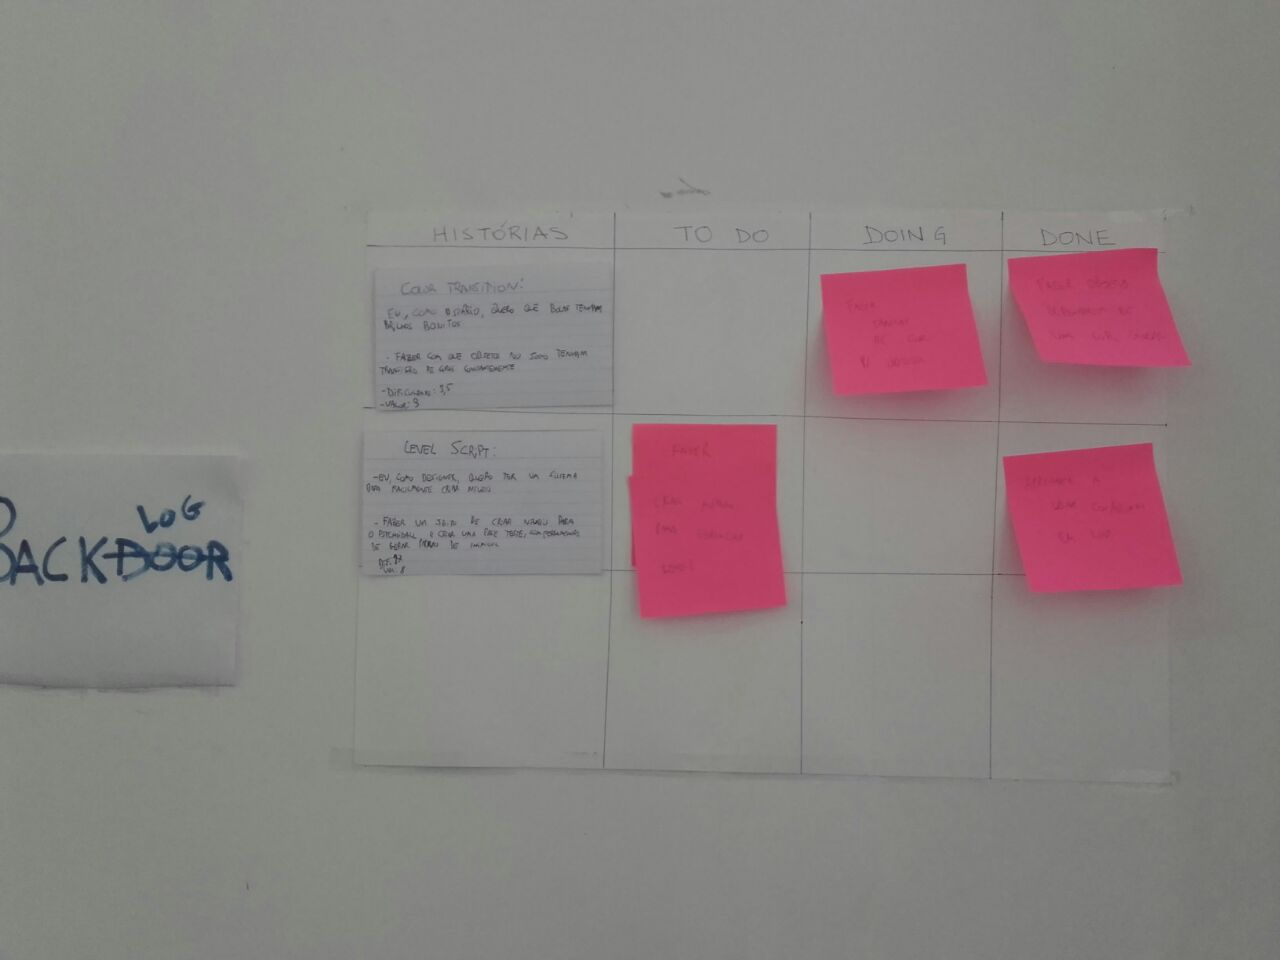
\includegraphics[scale=.3]{kanban}
\centering
\caption{Kanban utilizado durante o desenvolvimento de \textit{PsyChO: The Ball}}
\end{figure}

Entretanto, após alguns meses utilizando essa técnica, o tempo gasto em sua manutenção acabou se tornando mais trabalhoso do que produtivo para o projeto e seu uso foi decaindo. Desta forma o \textit{Kanban} foi substituido por várias pequenas técnicas ágeis, como lançamentos frequentes do jogo, \textit{sprints} (onde era determinado um prazo de uma ou duas semanas para terminar funcionalidades no jogo) e constante re-avaliação do jogo com consulta de \textit{feedback}.

Por último, uma técnica muito presente no desenvolvimento do jogo foi a utilização de documentação para marcar mudanças e melhorias no projeto. Os dois mais importantes são o \textit{DEVLOG}\footnote{https://github.com/uspgamedev/Project-Telos/blob/dev/docs/DEVLOG.md} e \textit{CHANGELOG}\footnote{https://github.com/uspgamedev/Project-Telos/blob/dev/docs/CHANGELOG.md}. O \textit{DEVLOG} foi um documento necessário para mostrar o progresso e tempo gasto no projeto, enquanto este fazia parte da disciplina \textit{MAC0214 Atividade Curricular em Cultura e Extensão}. Nele existe várias entradas detalhando atividades feitas no jogo durante o desenvolvimento. O documento \textit{CHANGELOG} por outro lado serve para marcar lançamentos do jogo, descrevendo \textit{features} novos adicionados em cada \textit{sprint} feito. Ambos documentos foram de grande utilidade no inicio do desenvolvimento de \textit{PsyChO: The Ball}, pois exibem concretamente o fluxo de progresso na criação do jogo.

% ---------------------------------------------------------------------------- %
\section{Ferramentas}
\label{sec:ferramentas}

Uma das escolha para o desenvolvimento de \textit{PsyChO: The Ball} foi a utilização exclusiva de \textit{Software Livre}. Essa escolha se deu tanto pela liberdade que essas ferramentas permitem em sua utilização, quanto pelo objetivo de incentivar mais o uso desse tipo de software, mostrando que são tão eficientes quanto o uso de software proprietários. Assim, como critério de escolha para cada área de desenvolvimento do jogo, foi determinado algum software livre que tenha uma comunidade ativa (para a solução de problemas e disponibilidade de bibliotecas), constante atualização de suas funcionalidades, versões estáveis e uma recomendação de seu uso no desenvolvimento de jogos.

O arcabouço utilizado no desenvolvimento do jogo foi a \textit{Love2d} ou \textit{LÖVE}\footnote{https://love2d.org/}, uma \textit{framework} grátis que utiliza a linguagem \textit{Lua}\footnote{https://www.lua.org/portugues.html}.

Como sistema de controle de versão foi utilizado \textit{Git}\footnote{https://git-scm.com/} através da plataforma de uso grátis \textit{Github}\footnote{https://github.com/}.

Para a produção de música foi utilizado \textit{LMMS}\footnote{https://lmms.io/}, um software livre grátis para manipulação e criação de sons.

Por último, para manipulação de imagens, foi utilizada a ferramenta \textit{Gimp}\footnote{https://www.gimp.org/}.

\begin{figure}[h!]

\includegraphics[scale=.5]{icons}
\centering
\caption{Da esquerda pra direita, ícones de \textit{LÖVE}, \textit{Lua}, \textit{Git}, \textit{Github}, \textit{LMMS} e \textit{Gimp}}
\end{figure}

Dentre essas ferramentas, vale ressaltar um ponto muito interessante do arcabouço \textit{LÖVE}. Seu \textit{gameloop} tem o diferencial de deslocar todos as verificações de \textit{input} do usuário como \textit{callbacks assíncronos}. Estes são funções que a própria \textit{framework} vai chamar quando ocorrer algum \textit{input} do usuário, como quando ele pressionar um botão do teclado ou mover o mouse. Através de subrotinas, o arcabouço está constantemente aguardando sinais que ativem essas funções e assim o desenvolvedor não precisa se preocupar em lidar com otimização ou código confuso na hora de esperar e tratar comandos dados pelo usuário. Isso foi uma grande vantagem que determinou a escolha dessa ferramenta na produção de \textit{PsyChO: The Ball}.

% ---------------------------------------------------------------------------- %
